\documentclass[10pt, landscape, a4paper]{article}

\usepackage{fontspec}
\usepackage[english]{babel}
\babelfont{rm}{Noto Sans}
\babelfont{sf}{Noto Sans}

\usepackage{amsmath}
\usepackage{amssymb}
\usepackage{hyperref}
\usepackage{url}
\usepackage{graphicx}
\usepackage{geometry}
\usepackage{enumitem}
\usepackage{parskip}
\usepackage{chemfig}
\usepackage{pdfpages}
\usepackage{xcolor}
\usepackage{tikz}
\usepackage{fancybox}
\usepackage{makecell}
\usepackage{pgfplots}
\usepackage{ulem}
\usepackage{wrapfig}
\usepackage{subcaption}
\usepackage{esvect}
\usepackage{siunitx}
\usepackage{mathtools}
\usepackage{varwidth}
\usepackage{multicol}
\usepackage{titlesec}

\usetikzlibrary{arrows}
\usetikzlibrary{arrows.meta}
\usetikzlibrary{decorations.pathreplacing}
\pgfplotsset{compat=1.18}
\definecolor{darkgreen}{rgb}{0.0, 0.6, 0.0}

% ============= GEOMETRY ADJUSTMENT =============
\geometry{
    a4paper,
    landscape,
    margin=1.5cm,
}

% ============= HEADER & TITLES =============
\usepackage{fancyhdr}
\pagestyle{fancy}
\fancyhf{}
\lhead{Systems Modelling}
\rhead{Matteo Frongillo}
\renewcommand{\headrulewidth}{0pt}

\titlespacing*{\section}{0pt}{8pt}{0pt}
\titlespacing*{\subsection}{0pt}{6pt}{2pt}
\titlespacing*{\subsubsection}{0pt}{4pt}{2pt}

\titleformat{\section}{\normalfont\Large\bfseries\color{black}}{}{0em}{}
\titleformat{\subsection}{\normalfont\large\bfseries\color[HTML]{007AFF}}{}{0em}{}
\titleformat{\subsubsection}{\normalfont\normalsize\bfseries\color[HTML]{007355}}{}{0em}{}

% ============= META DATA =============
\newcommand{\pdftitle}[1]{\hypersetup{
  colorlinks=true,
  linkcolor=black,
  urlcolor=blue,
  pdftitle={#1},
  pdfauthor={Matteo Frongillo}
}}

% ============= RENEW COMMANDS =============

\makeatletter
\renewcommand{\author}[1]{%
  \def\@author{%
    #1\\\\
    \parbox{\textwidth}{%
      \noindent
      \begin{minipage}[t]{0.15\textwidth}
        Last update:
      \end{minipage}%
      \begin{minipage}[t]{0.70\textwidth}
        \centering
        \today
      \end{minipage}%
      \begin{minipage}[t]{0.15\textwidth}
      \end{minipage}%
    }
  }%
}
\makeatother

\let\emptyset\varnothing

\makeatletter
\pgfmathdeclarefunction{arctan}{1}{%
    \begingroup
    \pgfmathparse{rad(atan(#1))}%
    \endgroup
}
\makeatother

% ============= NEW COMMANDS =============

\newcommand{\figbox}[1]{ 
    \begin{figure*}[ht!]        
        \begin{center}            
            \fbox{\begin{varwidth}{\textwidth} #1 \end{varwidth}}        
        \end{center}    
    \end{figure*}
}

\newcommand{\wrapfill}{
    \par
    \ifnum \value{WF@wrappedlines} > 0
        \addtocounter{WF@wrappedlines}{-1}%
        \null\vspace{
            \arabic{WF@wrappedlines}
            \baselineskip
        }
        \WFclear
    \fi
    \phantom{}
}

\ExplSyntaxOn
\DeclareDocumentCommand{\integral}{d[] d[] d[] d[]}
{
    \IfNoValueTF{#3}{
        \IfNoValueTF{#4}{
            \displaystyle \int #1\,d#2
        }{
            \text{Error: either 2 or 4 arguments must be provided}
        }
    }{
        \IfNoValueTF{#4}{
            \text{Error: either 2 or 4 arguments must be provided}
        }{
            \displaystyle
            \int\limits
                \IfNoValueF{#1}{\c_math_subscript_token{#1}}
                ^{\IfNoValueTF{#2}{}{#2}}
                #3\, d#4
        }
    }
}
\ExplSyntaxOff

\newcommand*\circled[1]{\tikz[baseline=(char.base)]{
            \node[shape=circle,draw,inner sep=2pt] (char) {#1};}}

\makeatletter
\newcommand*{\rom}[1]{\expandafter\@slowromancap\romannumeral #1@}
\makeatother

\newcommand{\difference}{\,\backslash\,}
\newcommand{\rem}{\underline{Remark}: }
\newcommand{\nots}{\underline{Notation}: }
\newcommand{\note}{\underline{Note}: }
\newcommand{\prf}{\underline{Proof}: }
\newcommand{\exs}{\underline{Example}: }
\newcommand{\defs}{\underline{Definition}: }
\newcommand{\wrn}{\underline{Warning}: }
\newcommand{\sht}{\ |\ }
\newcommand{\pph}[1]{\paragraph{#1} \phantom{}\\}
\newcommand{\dm}{\displaystyle}
\newcommand{\rad}{^{\mathrm{c}}}
\newcommand{\dsum}[2]{\displaystyle \sum_{#1}^{#2}}
\newcommand{\dx}[2]{\dfrac{{\mathrm{d}}^{#1}{#2}}{\mathrm{d}x^{#1}}}

% ============= DOCUMENT CONTENT =============

\title{Systems Modelling}
\author{Matteo Frongillo}
\date{\today}

\begin{document}

\setlength{\columnsep}{1cm}
\begin{multicols*}{3}

\section*{SW 1: Introduction}
\subsection*{Model's three properties}
\begin{itemize}
    \item[\textbf{Mapping}:] models act as a representation of natural or artificial originals and can be models in turn;
    \item[\textbf{Reduction}:] models function as abstraction. They do not capture every attribute of the original; instead, they isolate and retain only those attributes relevant to the spectific objective, intentionally omitting detail to manage complexity and focus on the problem at hand;
    \item[\textbf{Pragmatic}:] models function as utilitarian substitutes. They do not replace the original universally but serve as a representative for a specific user (subject), within a defined time frame, and for a particular purpose or operation.   
\end{itemize}

\textbf{Example}\\
\begin{center}
    \includegraphics[width=.75\linewidth]{media/sw1_inclinedplane.png}
\end{center}
\begin{itemize}
    \item[Generaliz.:] point mass sliding down an inclined plane;
    \item[Mapping:] box as mass, conveyor slope as an angle $\theta$, vertical drop as height $h$, gravity;
    \item[Reduction:] no structure flexibility, no air movement, no friction, no rollers\ $\rightarrow$\ flat plane;
    \item[Pragmatic:] it allows $a,v_f,t$ of the box to be calculated, it enables the prediction of how to build a belt mockup.  
\end{itemize}

\columnbreak
\subsection*{Digital representation}
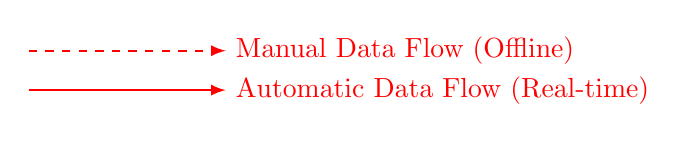
\begin{tikzpicture}
    \draw[-latex, dashed, thick, red] (0,0) -- (2.5,0) node[right] {Manual Data Flow (Offline)};
    \draw[-latex, thick, red] (0,-.5) -- (2.5,-.5) node[right] {Automatic Data Flow (Real-time)};
\end{tikzpicture}
\subsubsection*{Digital model (simulation)}
No direct connection between digital and physical object:
\begin{center}
    \includegraphics[width=.7\linewidth]{media/sw1_digitalmodel.png}
\end{center}

\subsubsection*{Digital shadow}
Unidirectional, automated data flow from physical object to digital model:
\begin{center}
    \includegraphics[width=\linewidth]{media/sw1_digitalshadow.png}
\end{center}

\subsubsection*{Digital twin}
Automated data exchange between physical object and model:
\begin{center}
    \includegraphics[width=.8\linewidth]{media/sw1_digitaltwin.png}
\end{center}

\subsection*{Role of time}
\subsubsection*{Stationary behavior}
Steady-state operation: $\dot{m}_\alpha = \dot{m}_\omega$

\subsubsection*{Dynamic behavior}
Non stationary/transient/unsteady: $\dfrac{dm}{dt} = \dot{m}_\alpha - \dot{m}_\omega$

\subsection*{Governing dynamics}
\subsubsection*{Empirical (black box)}
\begin{minipage}[c]{0.65\linewidth}
    Data based, without direct physics link.\\
    (ex: machine learning, fitting of functions)
\end{minipage}
\hfill
\begin{minipage}[c]{0.3\linewidth}
    \centering
    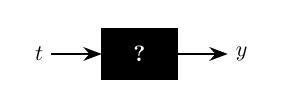
\begin{tikzpicture}[scale=0.8, every node/.style={scale=0.8}]
        \draw[thick, -{Stealth}] (-0.8, 0.4) -- (0, 0.4) node[pos=0, left] {$t$};
        \draw[thick, -{Stealth}] (1.2, 0.4) -- (2.0, 0.4) node[pos=1, right] {$y$};
        \draw[thick, fill=black] (0,0) rectangle (1.2,0.8);
        \node[white] at (0.6,0.4) {\textbf{?}};
    \end{tikzpicture}
\end{minipage}

\subsubsection*{Physics-based (white box)}
\begin{minipage}[c]{0.65\linewidth}
    Based on physical laws.\\
    (ex: conservation of mass)
\end{minipage}
\hfill
\begin{minipage}[c]{0.3\linewidth}
    \centering
    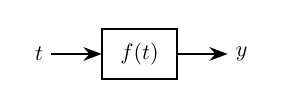
\begin{tikzpicture}[scale=0.8, every node/.style={scale=0.8}]
        \draw[thick, -{Stealth}] (-0.8, 0.4) -- (0, 0.4) node[pos=0, left] {$t$};
        \draw[thick, -{Stealth}] (1.2, 0.4) -- (2.0, 0.4) node[pos=1, right] {$y$};
        \draw[thick] (0,0) rectangle (1.2,0.8);
        \node at (0.6,0.4) {$f(t)$};
    \end{tikzpicture}
\end{minipage}

\subsubsection*{Grey-box (hybrid)}
\begin{minipage}[c]{0.65\linewidth}
    Combining physics and data\\ parameters.
\end{minipage}
\hfill
\begin{minipage}[c]{0.26\linewidth}
    \centering
    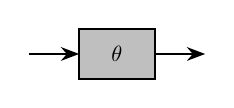
\begin{tikzpicture}[scale=0.8, every node/.style={scale=0.8}]
        \draw[thick, -{Stealth}] (-0.8, 0.4) -- (0, 0.4);
        \draw[thick, -{Stealth}] (1.2, 0.4) -- (2.0, 0.4);
        \draw[thick, fill=gray!50] (0,0) rectangle (1.2,0.8);
        \node at (0.6,0.4) {$\theta$};
    \end{tikzpicture}
\end{minipage}

\subsection*{Role of space}
\subsubsection*{Point model (0D)}
Assumes the whole system is perfectly mixed.\\
(ex: ideal mixer with isotropic distribution)\\
Software: Excel, MATLAB

\subsubsection*{Linked point}
Connects several simple models together to create a basic network or layout.\\
(ex: space shown via linking of 0D-models)\\
Software: Simulink, Modelica

\subsubsection*{Spatial model (1-3D)}
Considers real position of state variables or entities;
spatial relationships affect the dynamics.\\
(ex: real mixer with anisotropic, heterogeneous distribution)\\
Software: COMSOL, ANSYS, AutoCAD, REVIT

\textbf{Example with a heat pump}
\begin{itemize}
    \item Purpose: digital shadow $\to$\ automated data;
    \item Governing dynamics: physics-based\\$\to$\ based on thermodyn. laws;
    \item Time: time dependent, dynamic behavior $\to$\ heating load, power of the hp, on/off cycles;
    \item Space: linked point $\to$\ el. inputs, thermal\\energy exchange, 4 components to monitor.
\end{itemize}

\newpage
\subsection*{Solvability of models}
as example, $A=\integral[0][2][x^2][x]$
\subsubsection*{Analytical}
Closed formula as solution. Only for simple problems.
\[A=\dfrac{x^3}{3}\Big|_0^2 = \dfrac{8}{3}\]

\subsubsection*{Numerical}
Numerical approximation. For complex problems.
\[A\approx \dsum{i=1}{n} f(x_i) dx \approx 2.6667 \]

\subsection*{Further modelling properties}
\subsubsection*{Linear vs Non-linear}

\noindent
\begin{minipage}[t]{0.48\linewidth}
    \centering
    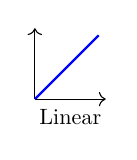
\begin{tikzpicture}[scale=0.45]
        \draw[->] (0,0) -- (2,0);
        \draw[->] (0,0) -- (0,2);
        \draw[blue, thick] (0,0) -- (1.8,1.8);
        \node[scale=.8] at (1,-0.5) {Linear};
    \end{tikzpicture}
\end{minipage}
\hfill
\begin{minipage}[t]{0.48\linewidth}
    \centering
    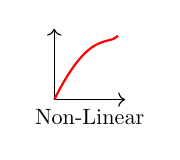
\begin{tikzpicture}[scale=0.45]
        \draw[->] (0,0) -- (2,0);
        \draw[->] (0,0) -- (0,2);
        \draw[red, thick] (0,0) .. controls (1,2) and (1.5,1.5) .. (1.8,1.8);
        \node[scale=.8] at (1,-0.5) {Non-Linear};
    \end{tikzpicture}
\end{minipage}

\subsubsection*{Continuity vs Differentiability}
\noindent
\begin{minipage}[t]{0.31\linewidth}
    \centering
    \scalebox{0.8}{
    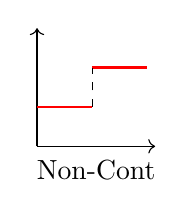
\begin{tikzpicture}
        \draw[->] (0,0) -- (1.5,0); \draw[->] (0,0) -- (0,1.5);
        \draw[red, thick] (0,0.5) -- (0.7,0.5);
        \draw[red, thick] (0.7,1.0) -- (1.4,1.0);
        \draw[dashed] (0.7,0.5) -- (0.7,1.0);
        \node at (0.75,-0.3) {Non-Cont};
    \end{tikzpicture}}
\end{minipage}
\hfill
\begin{minipage}[t]{0.31\linewidth}
    \centering
    \scalebox{0.8}{
    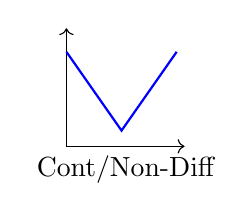
\begin{tikzpicture}
        \draw[->] (0,0) -- (1.5,0); \draw[->] (0,0) -- (0,1.5);
        \draw[blue, thick] (0,1.2) -- (0.7,0.2) -- (1.4,1.2);
        \node at (0.75,-0.3) {Cont/Non-Diff};
    \end{tikzpicture}}
\end{minipage}
\hfill
\begin{minipage}[t]{0.31\linewidth}
    \centering
    \scalebox{0.8}{
    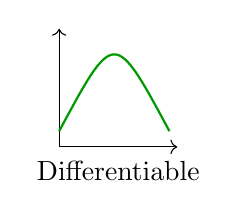
\begin{tikzpicture}
        \draw[->] (0,0) -- (1.5,0); \draw[->] (0,0) -- (0,1.5);
        \draw[darkgreen, thick] (0,0.2) .. controls (0.7,1.5) .. (1.4,0.2);
        \node at (0.75,-0.3) {Differentiable};
    \end{tikzpicture}}
\end{minipage}

\subsubsection*{Deterministic vs Stochastic}
\noindent
\begin{minipage}[t]{0.48\linewidth}
    \centering
    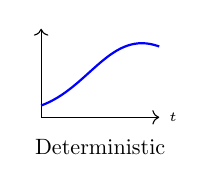
\begin{tikzpicture}[scale=0.75]
        \draw[->] (0,0) -- (2,0) node[right] {\tiny $t$};
        \draw[->] (0,0) -- (0,1.5);
        \draw[blue, thick] (0,0.2) to[out=20, in=160] (2,1.2);
        \node[scale=.8] at (1,-0.5) {Deterministic};
    \end{tikzpicture}
\end{minipage}
\hfill
\begin{minipage}[t]{0.48\linewidth}
    \centering
    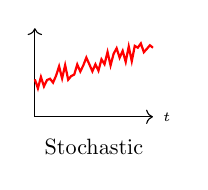
\begin{tikzpicture}[scale=0.75]
        \draw[->] (0,0) -- (2,0) node[right] {\tiny $t$};
        \draw[->] (0,0) -- (0,1.5);
        \draw[red, thick] plot[domain=0:2, samples=40] (\x, {0.6 + 0.3*\x + 0.15*rand});
        \node[scale=.8] at (1,-0.5) {Stochastic};
    \end{tikzpicture}
\end{minipage}

\subsection*{Modelling approaches}
\subsubsection*{Top-down}
Largest components broken down into smaller.\\
ex: marble block sculpture, railway network.\\
\circled{+} Efficient model, \circled{--} Misses details

\subsubsection*{Bottom-up}
Individual components combined into larger.\\
ex: LEGO model, human body.\\
\circled{+} Detailed model, \circled{--} Complex

\section{SW2: How to model a system}
\begin{enumerate}
    \item Problem formulation
    \item Mathematical representation
    \item Mathematical analysis
    \item Interpretation and evaluation of results
\end{enumerate}

\subsection*{Problem formulation}
\subsubsection{Task 1 - Defining goals}
What do we want to archieve?\\
How well/closely does our model need to represent reality?\\
What could be the goals for this specific system?

\subsubsection{Task 2 - Characterize the system}
What are the relevant parameters and variables of the system?\\
What are the system boundaries?\\
What are the inputs and outputs of the system?

\subsubsection*{Task 3 - Simplify and idealize the system}
Still reproduce the significant behaviors of the system, while reducing complexity.\\
Reduce model to the main parameters and variables (ex. for hp:
COP? Max. power? Avg power? Yearly values? Temperature levels?).

\subsection*{Mathematical formulation}
\subsubsection*{Task 1 - Identify fundamental theories and laws}
If no laws are available, use ad-hoc or empirical data to derive relationships:\\
Thermodynamic laws, material properties, ad-hoc $P_{out} = COP(T_{amb})\cdot P_{in}$

\subsubsection*{Task 2 - Derivation of relationships}
Derivation of relationships between the 


















\end{multicols*}

\end{document}